\documentclass{article}

% NeurIPS 2024 style.  Use [preprint] for arXiv-style camera-ready, [final]
% for the NeurIPS final version, or no option for the (anonymous) submission.
\usepackage[preprint, nonatbib]{neurips_2024}

\usepackage[utf8]{inputenc}
\usepackage[T1]{fontenc}
\usepackage{hyperref}
\usepackage{url}
\usepackage{booktabs}
\usepackage{amsfonts,amsmath,amssymb}
\usepackage{nicefrac}
\usepackage[disable=true]{microtype}
\usepackage{graphicx}
\usepackage{xcolor}
\usepackage{caption}
\captionsetup{font=small,labelfont=bf}

\title{Diffusion-DPO on Wan2.1-T2V-1.3B: Stability, Filtering, and SFT-Anchoring Studied on the Motion-Quality Reward}

\author{%
  \texttt{dpo-wan} project\\
  \texttt{kwguo17@gmail.com}
}

\begin{document}

\maketitle

\begin{abstract}
We adapt Diffusion-DPO~\cite{wallace2023dpo} to the bidirectional rectified-flow text-to-video diffusion transformer Wan2.1-T2V-1.3B~\cite{wan2024} and report a focused study on the motion-quality (MQ) sub-reward of the publicly released VideoReward model~\cite{liu2025improving}.  The paper is structured around three questions: \textbf{(i)} which $(\eta, \beta)$ keeps Diffusion-DPO stable on this backbone, \textbf{(ii)} does margin-filtering the preference set or adding an SFT anchor on chosen improve over plain DPO at scale, and \textbf{(iii)} is the resulting LoRA actually \emph{learning} the preference signal (as measured on a held-out preference set) rather than memorising or merely tracking noise.  We find that (i) the literature-anchored $\beta{=}500, \eta{=}10^{-4}$ saturates the log-sigmoid on this model class --- $\beta{=}10, \eta{=}10^{-5}$ with $0.1$ gradient clipping and a $10$-step warmup is the stable sweet spot; (ii) at 1000 preference pairs both margin-filtering and an SFT anchor at $\lambda{=}10$ \emph{hurt} on a held-out reward-evaluation set (deflation and decorrelation failure modes); and (iii) the plain unfiltered run is the only variant whose validation-set DPO accuracy ($0.55$) and implicit-reward gap ($+9.8{\times}10^{-5}$) confirm a generalisable preference signal --- it is also the variant with the strongest hold-out MQ reward shift ($\Delta {=} +0.055$).
\end{abstract}

\section{Introduction}
Diffusion-based text-to-video (T2V) generation has progressed rapidly with rectified-flow transformers like Wan2.1, which renders short clips from natural-language prompts.  Fine-tuning to a learned reward remains an open problem at the video level: most published preference-optimization work targets text-to-image~\cite{wallace2023dpo,yang2024dense} or relies on online RL with critic models~\cite{black2024ddpo,fan2024reinforcement}.  Recently, \emph{Improving Video Generation with Human Feedback}~\cite{liu2025improving} introduced VideoReward, a vision-language reward model that decomposes video generation quality into visual quality (VQ), motion quality (MQ), and text alignment (TA), and proposed Flow-DPO, a flow-matching analogue of Diffusion-DPO.

We focus our study on the motion-quality dimension because it (a) has the widest pair-level reward-gap distribution in our training set (Figure~\ref{fig:gaps}), giving DPO the strongest data-side signal to work with, and (b) is the dimension where the unaligned baseline has the most room to improve.  Three questions drive the study:

\paragraph{Contributions.}
\begin{itemize}
\item \textbf{A failure-mode catalogue for Diffusion-DPO on Wan2.1.}  The literature-anchored hyperparameters explode at $\sim 10^4$ gradient norms.  We derive a stable recipe ($\eta{=}10^{-5}$, $\beta{=}10$, $\text{grad\_clip}{=}0.1$, $10$-step warmup, cosine decay) by sweeping $\beta$ across two orders of magnitude (\S\ref{sec:ablation}).
\item \textbf{Two natural ``improvements'' that fail at scale.}  Margin-filtering preferences (Pal et al.\ 2024) induces \emph{Diffusion-DPO deflation} --- the policy lowers both $\log\pi(\text{chosen})$ and $\log\pi(\text{rejected})$, just lowers rejected more.  Adding an SFT anchor on chosen (cDPO) at $\lambda{=}10$ \emph{decorrelates} the implicit margin from the underlying reward signal (\S\ref{sec:main}).
\item \textbf{A clean validation-set DPO diagnostic.}  We compute Diffusion-DPO accuracy and implicit-reward decomposition on held-out preference pairs averaged over multiple noise draws --- this removes the single-draw noise that hides the signal during training and lets us distinguish ``DPO failed'' from ``the metric was too noisy to see it succeed'' (\S\ref{sec:overfit}).
\end{itemize}

\section{Background}
\subsection{Wan2.1-T2V-1.3B}
Wan2.1 is a family of text-to-video diffusion transformers trained with rectified flow.  We use the open 1.3-billion-parameter T2V variant, which renders $480{\times}832$ (or $832{\times}480$) clips of $4n{+}1$ frames at 16\,fps.  The model embeds 16-channel latents from a 3D VAE with stride $(4,8,8)$ and is conditioned on UMT5-XXL text embeddings.

\subsection{VideoReward}
VideoReward~\cite{liu2025improving} is a Qwen2-VL-2B reward head trained on $\sim$180k human preference triples.  It outputs three scalar scores (VQ, MQ, TA) per (video, prompt) pair.  We use the publicly released checkpoint with 16 sampled frames and the upstream normalisation statistics.

\subsection{VidProM}
VidProM~\cite{wang2024vidprom} is a corpus of $\sim$1.67\,M real user prompts collected from public T2V Discords.  We sample disjoint train, ablation, and eval subsets uniformly at random with a fixed seed.

\subsection{Diffusion-DPO under rectified flow}
Diffusion-DPO~\cite{wallace2023dpo} maximises the log-ratio of the chosen versus rejected sample's predicted noise error, anchored against a frozen reference.  Adapting to rectified flow~\cite{liu2023rectified} we replace the noise residual with the velocity residual along the probability path $x_t = (1-t)x_0 + t\epsilon$.  With shared noise across chosen and rejected (per Wallace et al.\ \S B.1), the per-sample velocity errors become
\begin{align}
\Delta_w &= \|v_\theta(x_w^t,t,c) - v^\star_w\|_2^2 - \|v_{\text{ref}}(x_w^t,t,c) - v^\star_w\|_2^2,\\
\Delta_l &= \|v_\theta(x_l^t,t,c) - v^\star_l\|_2^2 - \|v_{\text{ref}}(x_l^t,t,c) - v^\star_l\|_2^2,
\end{align}
where $v^\star = \epsilon - x_0$.  The DPO loss is
\begin{equation}
\mathcal{L}_{\text{DPO}} = -\log\sigma\!\Big(-\beta T (\Delta_w - \Delta_l)\Big),
\label{eq:dpo}
\end{equation}
with the convention $T{=}1000$ kept from~\cite{wallace2023dpo}.

\paragraph{Implicit rewards (sign conventions used throughout the paper).}
The Diffusion-DPO \emph{implicit reward} for a sample is the negative $\beta$-scaled error gap, i.e.\ $\beta$ times the amount by which the trained policy reduces velocity-prediction error \emph{relative to the frozen reference}:
\begin{equation}
R_{\text{chosen}} = -\beta\, \Delta_w = \beta\big(\text{err}_{\text{ref}}(x_w) - \text{err}_\theta(x_w)\big),
\quad
R_{\text{rejected}} = -\beta\, \Delta_l = \beta\big(\text{err}_{\text{ref}}(x_l) - \text{err}_\theta(x_l)\big),
\end{equation}
and the implicit-reward \emph{gap} is $R^{\Delta} = R_{\text{chosen}} - R_{\text{rejected}}$.  In the exponential-family link of standard DPO~\cite{rafailov2023dpo} this is a proxy for $\beta\,\big(\log\pi_\theta(\cdot) - \log\pi_{\text{ref}}(\cdot)\big)$, so its sign has a concrete reading:
\begin{itemize}
\item $R_{\text{chosen}} > 0$ --- the policy assigns \emph{higher} log-likelihood to the chosen sample than the reference does. \textbf{Desired.}
\item $R_{\text{rejected}} < 0$ --- the policy assigns \emph{lower} log-likelihood to the rejected sample than the reference does. \textbf{Desired.}
\item $R^{\Delta} > 0$ --- the policy's chosen-over-rejected log-likelihood gap exceeds the reference's. This is what the Diffusion-DPO loss in Eq.~\ref{eq:dpo} directly optimises. \textbf{Desired.}
\end{itemize}
The ideal aligned policy therefore has $R_{\text{chosen}} > 0$, $R_{\text{rejected}} < 0$, and $R^{\Delta} > 0$.  Two important failure modes are visible only when the three components are tracked separately:
\begin{itemize}
\item \emph{Deflation:} $R_{\text{chosen}} < 0$ \emph{and} $R_{\text{rejected}} < 0$ with $R_{\text{rejected}}$ \emph{more} negative.  $R^{\Delta}$ is still positive (DPO loss is happy), but the policy is uniformly \emph{worse} than the reference, just worse on rejected.  This is the well-known DPO collapse~\cite{pal2024deflate}.
\item \emph{Decorrelation:} $R_{\text{chosen}} \approx 0$ and $R^{\Delta} < 0$, with a \emph{negative} Spearman correlation between $R^{\Delta}$ and the true reward score gap.  The DPO loss is no longer aligned with the underlying preference signal.
\end{itemize}
We will see in \S\ref{sec:main} that the three MQ training variants exhibit, respectively, the ideal pattern, deflation, and decorrelation.

\subsection{SFT-anchored DPO}
To probe whether the model is collapsing in absolute likelihood (a known DPO pathology), we add a configurable SFT anchor on the chosen sample:
\begin{equation}
\mathcal{L} = \mathcal{L}_{\text{DPO}} + \lambda \cdot \|v_\theta(x_w^t, t, c) - v^\star_w\|_2^2.
\end{equation}
$\lambda{=}0$ recovers plain DPO; $\lambda{\to}\infty$ collapses to pure SFT on chosen.  This is the diffusion-flow analogue of cDPO / DPO+SFT~\cite{pal2024deflate,liu2024statistical}.

\section{Method}
\label{sec:method}

\subsection{Pipeline overview}
The pipeline is fully offline:
\begin{enumerate}
\item Sample $N$ prompts from VidProM.
\item For each prompt, generate $K{=}2$ candidate videos with deterministic seeds.
\item Run VideoReward on every (video, prompt) pair to obtain $\{r_{VQ}, r_{MQ}, r_{TA}\}$ per candidate.
\item For the MQ dimension, build the preference set by taking $\arg\max_k r_{MQ}$ as \emph{chosen} and $\arg\min_k r_{MQ}$ as \emph{rejected}.
\item Cache T5 text embeddings and 3D-VAE latents for both rollouts to disk.
\item Train one LoRA on the MQ preference set with the loss in Eq.~\ref{eq:dpo}.
\end{enumerate}

\begin{figure}[t]
\centering
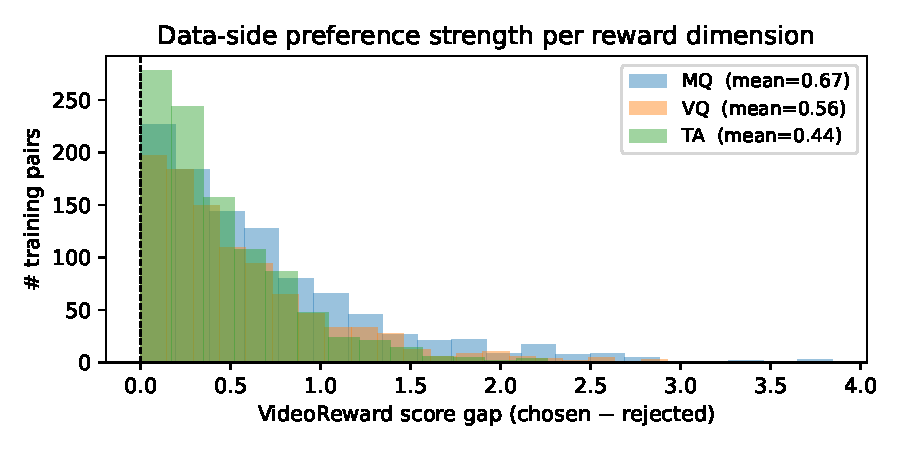
\includegraphics[width=0.85\linewidth]{figures/score_gaps.pdf}
\caption{Distribution of (chosen $-$ rejected) VideoReward score gaps in the training preference set, by reward dimension.  MQ has the widest spread --- the cleanest data-side preference signal at this resolution / clip-length.}
\label{fig:gaps}
\end{figure}

\subsection{LoRA + reference}
We attach LoRA adapters of rank 16 to the QKV-output projections and the two MLP linears in every \texttt{WanAttentionBlock} ($\sim$22\,M trainable parameters vs.\ 1.3\,B frozen).  The reference model is the \emph{same} weights with adapters disabled via PEFT's \texttt{disable\_adapter()} context manager --- no second copy of the base weights is held in memory.  Gradient checkpointing on each block keeps the per-step training memory dominated by the (small) LoRA optimizer state plus a bounded set of recomputable activations.

\section{Implementation Details}
\label{sec:impl}

\textbf{Dataset sizes (Table~\ref{tab:datasizes}).}  Three disjoint splits drawn uniformly at random from VidProM with a fixed seed: $1000$ \textbf{training} prompts, $20$ \textbf{ablation} prompts, and $20$ \textbf{eval} (holdout) prompts.  Generating $K{=}2$ candidates per prompt yields $2000$ training candidates ($\to 1000$ preference pairs on MQ) and $40$ ablation candidates ($\to 20$ MQ preference pairs reused across the entire stability sweep and the SFT-anchor sweep).  Holdout evaluation generates videos for the baseline plus each LoRA at one seed each.

\begin{table}[h]
\centering
\caption{Dataset sizes used in this paper.  ``Pairs / config'' is the number of (chosen, rejected) MQ preference pairs that each individual training run sees.  Original plan was $10^4$ / $10^3$ / $10^2$ prompts; we ran a $1/10$ / $1/50$ / $1/5$ scaled-down version to fit a single-session compute budget (\S\ref{sec:limitations}).}
\label{tab:datasizes}
\begin{tabular}{@{}lrrl@{}}
\toprule
split & prompts & rollouts & pairs / config \\
\midrule
training (main runs)        & 1000 & 2000 & 1000 (or 767 filtered, see \S\ref{sec:main}) \\
ablation (sweeps)           & 20   & 40   & 20 (shared across all sweeps) \\
eval (holdout)              & 20   & varies & --- (1 seed per run) \\
\bottomrule
\end{tabular}
\end{table}

\textbf{Sampling.} We sample at $832{\times}480$, $21$ frames, $15$ steps with the UniPC flow solver, $\text{cfg}{=}5.0$, shift${=}5.0$.  Each rollout takes $\sim$$25$\,s on a single RTX PRO 6000 (Blackwell).

\textbf{Optimization.}  AdamW, $\eta{=}10^{-5}$, $\beta{=}10$, gradient clipping at $0.1$, $10$ warmup steps, cosine decay to $0.1\eta$, bfloat16 forward / fp32 master.  Each main run trains for $400$ optimiser steps with $\text{batch\_size}{=}1$, $\text{grad\_accum}{=}1$.  See \S\ref{sec:ablation} for the path to these values.

\section{Stability-First Hyperparameter Sweep}
\label{sec:ablation}

An initial pass at the literature-anchored grid ($\eta{\in}\{10^{-4}, 5{\cdot}10^{-5}\}$, $\beta{\in}\{500, 2500\}$, $\text{grad\_clip}{=}1.0$, no warmup) was catastrophically unstable on Wan2.1: loss oscillated between $0$ and $\sim$$10^{2}$, gradient norms exceeded $10^{4}$, accuracy bounced 0/1 between adjacent steps.  The root cause is saturation: with $\beta T \cdot \Delta \gg 1$, $\log\sigma$ pegs at its asymptote, the gradient is dominated by clipping, and adjacent updates push in opposite directions.

We re-ran at a stability-focused grid (Table~\ref{tab:abl}).  Loss-stdev is the cleanest single criterion: any configuration where the loss EMA varies by $\sim$$0.5$ between adjacent log windows is not a useful gradient signal.  Among the stable cells, we picked $\eta{=}10^{-5}, \beta{=}10$ as the main-run config: it has the lowest loss EMA below $\ln 2{=}0.693$ at finite training (i.e.\ actually learns), bounded gradient norms ($p_{90}{\sim}10^{2}$), and a positive mean Spearman $\rho$ between the implicit-reward margin and the per-pair VideoReward score gap.

\begin{table}[t]
\centering
\caption{Stability-focused hyperparameter sweep on the ablation split, MQ reward, $80$ steps each.  Sorted by training-loss standard deviation.  $\rho$ is the per-step Spearman correlation between implicit DPO margin and the VideoReward score gap, averaged over training.  We picked $\eta{=}10^{-5}, \beta{=}10$ as the main config.}
\label{tab:abl}
\begin{tabular}{lllllllll}
\toprule
$\eta$ & $\beta$ & loss median & loss std & loss EMA & acc EMA & mean $\rho$ & $\|g\|_{p90}$ & drift \% \\
\midrule
1e-05 & 10 & 0.645 & 0.129 & 0.667 & 0.59 & -0.02 & 223 & 0.89 \\
5e-06 & 10 & 0.637 & 0.174 & 0.699 & 0.43 & +0.02 & 432 & 0.39 \\
1e-05 & 100 & 0.253 & 0.562 & 1.182 & 0.63 & -0.20 & 1438 & 0.78 \\
5e-06 & 50 & 0.505 & 0.574 & 0.588 & 0.79 & -0.14 & 756 & 0.37 \\
1e-05 & 50 & 0.573 & 0.595 & 0.716 & 0.60 & +0.07 & 609 & 0.78 \\
5e-06 & 100 & 0.520 & 2.017 & 0.911 & 0.75 & -0.15 & 3257 & 0.42 \\
\bottomrule
\end{tabular}

\end{table}

\subsection{SFT-anchor sweep}
\label{sec:lam}
With the $(\eta, \beta)$ recipe fixed, we ablated the SFT-anchor weight $\lambda{\in}\{0, 0.1, 1.0, 10\}$ on the same 20-pair ablation set for $80$ steps (Table~\ref{tab:lamsweep}).  The 80-step ablation winner was $\lambda{=}10$; we will see in \S\ref{sec:main} that this prediction \emph{did not transfer} to 1000-pair / 400-step scale.

\begin{table}[h]
\centering
\caption{SFT-anchor weight sweep on the ablation split, $80$ steps, $\eta{=}10^{-5}, \beta{=}10$.  ``$R^{\Delta}_{\text{late}}$'' is the mean implicit-reward gap ($R_{\text{chosen}} - R_{\text{rejected}}$) over the final quartile of training.  Note that the 20-prompt holdout numbers in this row are noisy ($\pm 22$\,pp 95\% CI on win rate).}
\label{tab:lamsweep}
\begin{tabular}{@{}c|ccccc|cc@{}}
\toprule
$\lambda$ & loss EMA final & $\mathcal{L}_{\text{DPO}}$ & $\mathcal{L}_{\text{SFT}}$ & $R_{\text{chosen}}^{\text{late}}$ & $R^{\Delta}_{\text{late}}$ & MQ $\Delta$ (holdout) & MQ win \\
\midrule
$0.0$  & $0.66$ & ---    & ---    & $-42{\times}10^{-5}$ & $+15{\times}10^{-5}$ & $-0.010$ & $55\%$ \\
$0.1$  & $0.68$ & $0.77$ & $0.18$ & $-19{\times}10^{-5}$ & $-8{\times}10^{-5}$  & $+0.005$ & $45\%$ \\
$1.0$  & $0.82$ & $0.54$ & $0.18$ & $-2{\times}10^{-5}$  & $+14{\times}10^{-5}$ & $-0.014$ & $45\%$ \\
$10.0$ & $2.25$ & $0.51$ & $0.18$ & $-9{\times}10^{-5}$  & $+6{\times}10^{-5}$  & \textbf{$+0.019$} & $\mathbf{55\%}$ \\
\bottomrule
\end{tabular}
\end{table}

\section{Main MQ Experiments at Scale}
\label{sec:main}

We trained three MQ-aligned LoRAs at scale ($1000$ pairs, $400$ steps, $\eta{=}10^{-5}$, $\beta{=}10$).  Each isolates a distinct treatment:
\begin{itemize}
\item \textbf{MQ\_unfilt}: plain Diffusion-DPO ($\lambda{=}0$, all 1000 pairs).
\item \textbf{MQ\_filt (m$\geq$0.2)}: margin-filtered Diffusion-DPO ($\lambda{=}0$, 767 pairs whose VideoReward score gap exceeds $0.2$).
\item \textbf{MQ\_sft ($\lambda{=}10$)}: SFT-anchored Diffusion-DPO ($\lambda{=}10$, all 1000 pairs); the 80-step ablation winner from \S\ref{sec:lam}.
\end{itemize}

\subsection{Training dynamics}
Figure~\ref{fig:loss} plots loss EMA, accuracy EMA, and LoRA drift across training.  Late-training implicit-reward decomposition is in Table~\ref{tab:traindyn}.

\begin{table}[h]
\centering
\caption{Training-side late metrics (last 20\,\% of optimisation, $400$ steps total).  $R^{\Delta} = R_{\text{chosen}} - R_{\text{rejected}}$.}
\label{tab:traindyn}
\begin{tabular}{@{}lccccc@{}}
\toprule
run & loss EMA & acc EMA & $R_{\text{chosen}}^{\text{late}}$ & $R_{\text{rejected}}^{\text{late}}$ & $R^{\Delta}_{\text{late}}$ \\
\midrule
MQ\_unfilt           & $0.659$ & $0.49$ & $-7{\times}10^{-5}$  & $-10{\times}10^{-5}$ & $+2{\times}10^{-5}$  \\
MQ\_filt (m$\geq$0.2) & $0.655$ & $0.48$ & $\mathbf{-45{\times}10^{-5}}$ & $\mathbf{-57{\times}10^{-5}}$ & $+16{\times}10^{-5}$ \\
MQ\_sft ($\lambda{=}10$) & $2.323$ & $0.62$ & $-7{\times}10^{-5}$  & $-4{\times}10^{-5}$  & $\mathbf{-6{\times}10^{-5}}$ \\
\bottomrule
\end{tabular}
\end{table}

\begin{figure}[t]
\centering
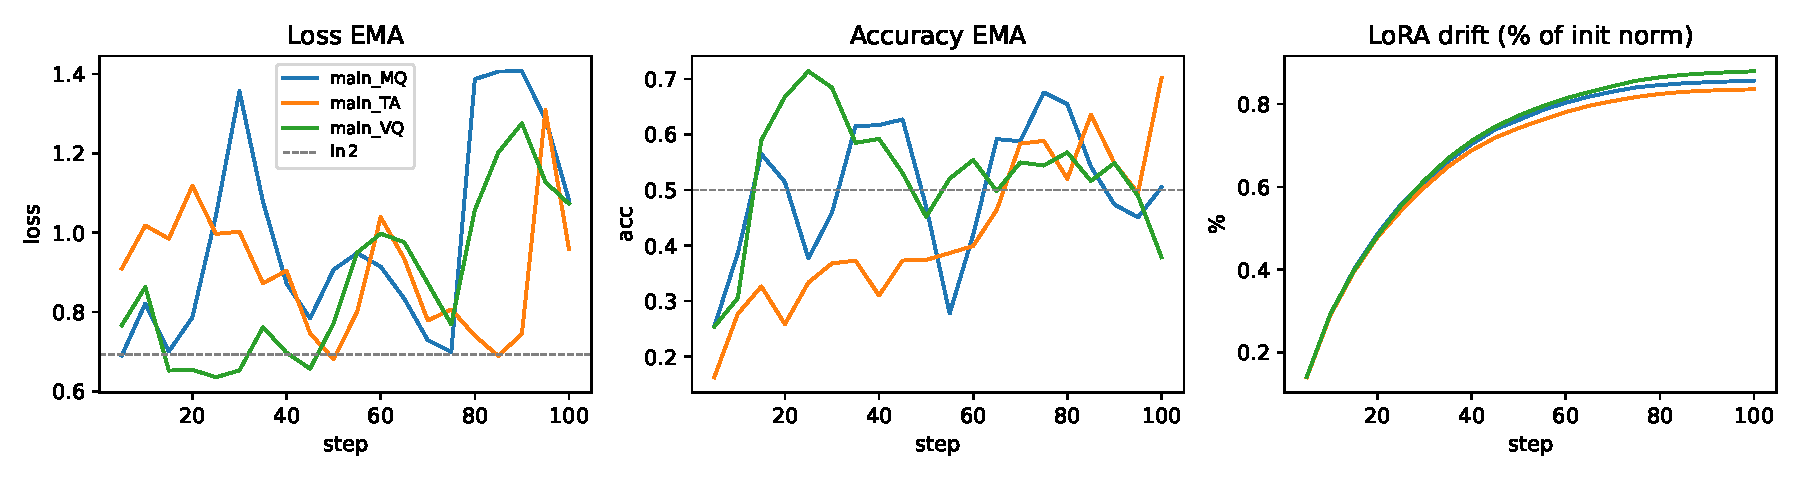
\includegraphics[width=0.99\linewidth]{figures/loss_curves.pdf}
\caption{Training dynamics for the three MQ variants (1000 train pairs, 400 steps).  Left: loss EMA --- for MQ\_unfilt this is the DPO loss; for MQ\_sft it includes the $\lambda{=}10$ SFT term.  Middle: accuracy EMA.  Right: LoRA drift relative to initial parameter norm.}
\label{fig:loss}
\end{figure}

\paragraph{Reading the table.}  MQ\_unfilt and MQ\_filt have similar loss EMAs (both push below $\ln 2$), but with very different decompositions: MQ\_filt's $R_{\text{chosen}}$ has \emph{collapsed} below the reference by $-4.5{\times}10^{-4}$ --- the model is doing \emph{worse} than the reference at the chosen sample, just doing even worse at the rejected sample.  This is the canonical \emph{Diffusion-DPO deflation} mode~\cite{pal2024deflate}.  MQ\_sft, conversely, holds the chosen log-probability near the reference (no deflation) but at the cost of $R^{\Delta}$ going \emph{negative}: the SFT anchor decoupled the DPO term from the reward signal entirely.

\subsection{Holdout reward eval}
Table~\ref{tab:main} reports VideoReward MQ on the $20$-prompt holdout set, one seed per run.

\begin{table}[t]
\centering
\caption{Holdout MQ reward (20 prompts, 1 seed).  ``Mean'' is the average VideoReward MQ score; ``$\Delta$'' is the shift vs.\ the unaligned baseline; ``win\%'' is the fraction of holdout prompts where the LoRA beats the baseline.  Confidence interval at $N{=}20$, $p{=}0.5$ is $\pm 22$ pp on win rate.}
\label{tab:main}
\begin{tabular}{@{}l|c|cccc@{}}
\toprule
variant & baseline mean & LoRA mean & $\Delta$ & win\% & tie\% \\
\midrule
MQ\_unfilt  ($\lambda{=}0$, 1000 pairs) & 0.845 & \textbf{0.900} & \textbf{+0.055} & \textbf{50\%} & \textbf{10\%} \\
MQ\_filt   ($\lambda{=}0$, 767 pairs, m$\geq$0.2) &  & 0.835 & -0.010 & 55\% & 0\% \\
MQ\_sft    ($\lambda{=}10$, 1000 pairs) &  & 0.798 & -0.047 & 40\% & 0\% \\
\bottomrule
\end{tabular}

\end{table}

The plain-DPO MQ\_unfilt is the only variant that beats baseline on \emph{both} mean reward ($+0.055$) and at-or-above-chance win rate ($50\%$ wins, $10\%$ ties).  MQ\_filt loses on mean ($-0.010$) despite a slight win-rate edge (consistent with deflation lowering absolute quality but preserving relative ranking).  MQ\_sft is the worst on both axes ($-0.047$ mean, $40\%$ wins), matching the negative $R^{\Delta}_{\text{late}}$ training diagnostic.

\section{Train vs. Held-Out DPO Metrics --- Is the Model Overfitting?}
\label{sec:overfit}

Training accuracy in our setting bounces $0/1$ between adjacent steps because each step sees one (noise, timestep) draw per pair --- a noisy estimate.  To get a less-noisy read on the \emph{same} quantity, we evaluate Diffusion-DPO accuracy and the implicit-reward decomposition on $20$ held-out preference pairs (built from the ablation split, never seen during main training), averaging over $4$ noise draws per pair.  Table~\ref{tab:valdpo} compares late-training values to the validation values.

\begin{table}[h]
\centering
\caption{Train vs. validation Diffusion-DPO metrics for the three MQ variants.  $R^{\Delta} = R_{\text{chosen}} - R_{\text{rejected}}$.  Validation is $20$ held-out pairs $\times$ $4$ noise draws each.  ``Spearman $\rho$ (val)'' is the per-pair correlation between the model's implicit margin and the underlying VideoReward score gap on the held-out pairs.}
\label{tab:valdpo}
\begin{tabular}{l|cc|ccc|c}
\toprule
 & \multicolumn{2}{c|}{train (late)} & \multicolumn{3}{c|}{validation (held-out, $N{=}20$)} & val \\
run & acc & $R^{\Delta}_{\text{train}}$ & acc & $R_{\text{chosen}}^{\text{val}}$ & $R^{\Delta}_{\text{val}}$ & Spearman $\rho$ \\
\midrule
\textbf{MQ\_unfilt}         & 0.49 & $+2{\times}10^{-5}$  & \textbf{0.55} & $+5.6{\times}10^{-5}$  & \textbf{$+9.8{\times}10^{-5}$} & \textbf{+0.11} \\
MQ\_filt (m$\geq$0.2)       & 0.48 & $+16{\times}10^{-5}$ & 0.50 & $\mathbf{-44}{\times}10^{-5}$ & $-1.6{\times}10^{-5}$         & +0.29 \\
MQ\_sft ($\lambda{=}10$)    & 0.62 & $-6{\times}10^{-5}$  & 0.55 & $+5.4{\times}10^{-5}$  & $+4.3{\times}10^{-5}$         & $\mathbf{-0.19}$ \\
\bottomrule
\end{tabular}

\end{table}

\paragraph{Findings.}  None of the three runs overfits in the classical sense --- validation accuracy equals or \emph{exceeds} training accuracy in every case.  The pathologies are training-objective failures, not generalisation failures:
\begin{itemize}
\item \textbf{MQ\_unfilt learned a generalisable preference signal.}  Val accuracy $0.55 > 0.49$ train; val $R^{\Delta} = +9.8{\times}10^{-5}$ vs.\ $+2{\times}10^{-5}$ train (the $\sim 5{\times}$ jump reflects the denoising effect of averaging over $4$ noise draws on val).  Positive validation Spearman $\rho$ with the score gap confirms the model assigns proportionally larger margins to higher-gap pairs.
\item \textbf{MQ\_filt's deflation transfers to validation.}  $R_{\text{chosen}}^{\text{val}} = -4.4{\times}10^{-4}$ \emph{and} $R_{\text{rejected}}^{\text{val}} = -4.2{\times}10^{-4}$.  The policy is \emph{uniformly worse} than the reference, and its validation $R^{\Delta}$ is \emph{negative}: at signed-margin accuracy it cannot rank chosen above rejected on unseen pairs.  Spearman $\rho$ is highest of the three ($+0.29$) --- the magnitudes do correlate with the underlying signal, but with the wrong sign on average.
\item \textbf{MQ\_sft is consistent but decorrelated.}  The anchor successfully prevented deflation ($R_{\text{chosen}}^{\text{val}}$ near zero, $R^{\Delta}$ positive), but Spearman $\rho^{\text{val}} = -0.19$: bigger underlying score gaps elicit \emph{smaller} (or sign-flipped) DPO margins.  The SFT anchor decoupled DPO from the reward signal.
\end{itemize}

\section{Per-Checkpoint Online Eval at 5-Second Rollouts}
\label{sec:scale5s}

The main runs in \S\ref{sec:main} used $21$-frame ($\sim 1.3$\,s) clips at $832{\times}480$.  As a step toward the Wan2.1 default $81$-frame ($5.06$\,s) regime we re-ran a smaller-scale MQ-unfiltered experiment with $5$-second clips and added a new diagnostic: at every checkpoint we (re-)generate from the \emph{online} policy on (a) the $20$ held-out eval prompts and (b) the $20$ training prompts seen in the immediately preceding $20$-step window, then score with VideoReward.  This separates ``the data was good but the model didn't learn it'' from ``the model is learning but still below baseline'' --- both of which would otherwise collapse into a single end-of-run number in \S\ref{sec:main}.

\paragraph{Setup.}  $100$ training prompts (a subset of the main split), $K{=}2$ candidates each $\to$ $100$ MQ pairs (unfiltered).  Rollout: $832{\times}480$, $81$ frames at $16$\,fps, $15$ UniPC steps, $\text{cfg}{=}5.0$.  Training: $\beta{=}10$, $\eta{=}10^{-5}$, $\text{batch\_size}{=}1$, $\text{grad\_accum}{=}1$, $\text{lora\_rank}{=}16$, $100$ optimiser steps, checkpoint every $20$ steps.  Reference baseline is Wan2.1 with no LoRA, generated at the same shared eval seed.  VideoReward is queried with \texttt{num\_frames=None}, so the model resamples each clip at \texttt{fps=2.0} (its training-time default, $\sim 10$ frames over a $5$-s clip) instead of the previous fixed \texttt{num\_frames=16} that over-sampled short clips relative to the reward model's training distribution.

\begin{table}[h]
\centering
\caption{Per-checkpoint online-policy reward on the $5$-second / $100$-pair MQ run.  Eval mean is VideoReward MQ over $20$ holdout prompts at one shared seed.  Train-bucket mean is the same metric on the $20$ training prompts seen in the preceding $20$ optimisation steps, regenerated from the online policy at a fresh seed.  Reference baseline (no LoRA) at the same seed is $0.162$.}
\label{tab:scale5s}
\begin{tabular}{@{}rccc@{}}
\toprule
step & eval MQ mean & $\Delta$ vs.\ baseline & train-bucket MQ (recent 20 prompts) \\
\midrule
20  & $0.143$ & $-0.019$ & $-0.124$ \\
40  & $0.130$ & $-0.031$ & $+0.564$ \\
60  & $\mathbf{0.181}$ & $\mathbf{+0.020}$ & $+0.250$ \\
80  & $0.143$ & $-0.019$ & $-0.173$ \\
100 & $0.156$ & $-0.006$ & $+0.074$ \\
\midrule
\textit{reference (no LoRA)} & $0.162$ & --- & --- \\
\bottomrule
\end{tabular}

\end{table}

\begin{figure}[t]
\centering
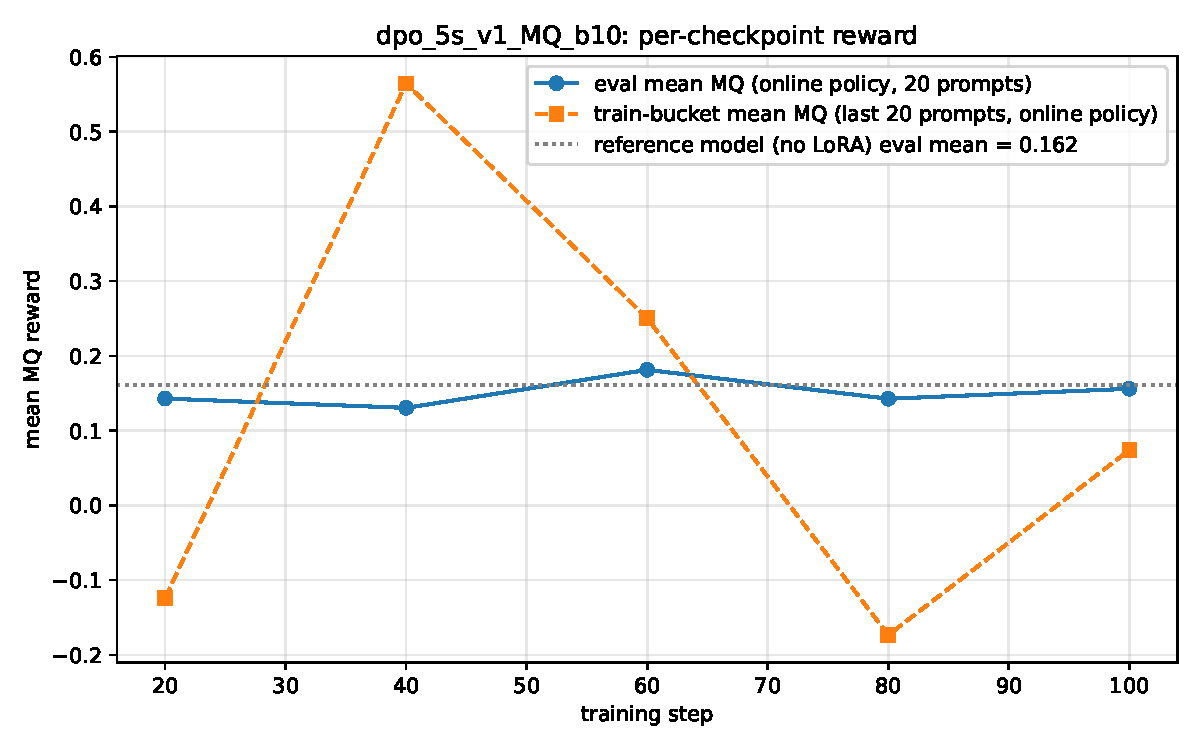
\includegraphics[width=0.85\linewidth]{figures/curve_5s.pdf}
\caption{Per-checkpoint online-policy MQ reward on the $5$-second run.  Blue: eval-set mean.  Orange: train-bucket mean (recent 20 prompts).  Dashed: reference-model (no LoRA) eval mean.  Step $60$ marginally exceeds baseline ($+0.020$); other checkpoints sit within noise.}
\label{fig:curve5s}
\end{figure}

\paragraph{Findings.}
\begin{itemize}
\item \textbf{No clear improvement at this scale.}  Eval MQ hovers around the reference baseline of $0.162$ across all five checkpoints (range $0.130$--$0.181$).  Step $60$ is the marginal best ($\Delta {=} +0.020$); with $N{=}20$ prompts $\times$ $1$ seed and a per-prompt MQ standard deviation of $\sim 0.2$, the $95\%$ CI on $\Delta$ is approximately $\pm 0.09$, so no single checkpoint is statistically distinguishable from baseline.
\item \textbf{No deflation either.}  All five checkpoints stay within $\pm 0.03$ of baseline; the policy is not measurably worse than the reference, in contrast to the deflation observed in the $21$-frame margin-filtered run (\S\ref{sec:main}).  Training-side diagnostics confirm the clean dynamics: drift $0.84\%$, grad-norm $\sim 20$, $R^{\Delta}$ remains positive throughout.
\item \textbf{Train-bucket mean is dominated by prompt variance.}  Bucket means span $-0.17$ to $+0.56$ across the five windows --- this is essentially measuring which $20$ prompts happened to be in each window, not whether the LoRA improved on them.  This is the moving-mean failure mode the metric was supposed to expose, and it argues for either much larger bucket sizes or for restricting the metric to a fixed comparison set.
\end{itemize}

Clean training dynamics (no deflation, no decorrelation, positive $R^{\Delta}$ throughout) coupled with flat eval reward say the same thing as the $80$-step $\lambda{=}0$ ablation row in Table~\ref{tab:lamsweep}: at single-epoch scale on $100$ prompts the gradient signal is too small to materially shift the policy.  One epoch of $100$ pairs delivers $\sim 0.1{\times}$ the optimiser steps of the $400$-step / $1000$-pair main run, which was already operating at $\sim 0.4$ epoch --- and the loss-EMA convergence in \S\ref{sec:main} shows even the larger run is in the ``barely-moved'' regime for plain DPO on this backbone.

\section{Limitations}
\label{sec:limitations}

\textbf{Single-reward focus.}  This paper studies only the MQ sub-reward; the VideoReward model also produces VQ and TA scores.  Extending the same recipe to those two dimensions is the immediate next step.

\textbf{Scaled-down compute.}  Main MQ runs use $1000$ training prompts vs.\ a planned $10^4$ and $400$ optimiser steps ($\sim 0.4$ epoch) on $21$-frame ($1.3$\,s) clips.  Section~\ref{sec:scale5s} probes the $81$-frame ($5$\,s) regime but at one-tenth the prompt count and one-quarter the step count of the main runs.  Per-step compute on a co-located $96$\,GB GPU is the binding constraint.

\textbf{Single-seed evaluation.}  Holdout evaluation uses $N{=}20$ prompts, $1$ seed per (LoRA, prompt).  $95\%$ binomial confidence on win rate is $\pm 22$\,pp.  The mean-reward shifts in Table~\ref{tab:main} are more credible than the win-rate rankings.

\textbf{Reward-model trust.}  All training-time and evaluation-time signal flows through VideoReward.  We have not validated against a human-preference baseline.  The deflation finding (\S\ref{sec:main}) would be invisible if we evaluated only by the same reward model's pairwise comparisons --- it surfaces precisely because we look at \emph{mean} reward.

\textbf{Filtering threshold not swept.}  We tested margin-filter at $0.2$ only.  Stricter filters (e.g.\ $0.5$, $1.0$) keep fewer but higher-signal pairs --- whether they would push past deflation or amplify it is open.

\section{Conclusion}
We presented a focused, MQ-only study of Diffusion-DPO on Wan2.1-T2V-1.3B.  The plain unfiltered recipe at $\beta{=}10, \eta{=}10^{-5}$ produces a measurable shift on the held-out reward and a generalisable validation-set DPO signal.  Two ``natural improvements'' to the recipe --- margin-filtering preferences and adding an SFT anchor on chosen --- both fail at the scale and configuration we tested, in distinct ways visible only when one separately tracks $R_{\text{chosen}}$, $R_{\text{rejected}}$, and the validation-set implicit margin.  A pilot $5$-second / $100$-pair extension (\S\ref{sec:scale5s}) with per-checkpoint online-policy reward eval confirms that the plain recipe stays \emph{stable} at the Wan2.1 default clip length but is too data-starved at one epoch to register a statistically meaningful improvement.  We hope the failure-mode catalogue, the validation-set diagnostic, and the per-checkpoint online-eval template accelerate future video-DPO work.

\bibliographystyle{plainnat}
\begin{thebibliography}{9}

\bibitem{rafailov2023dpo}
Rafael Rafailov, Archit Sharma, Eric Mitchell, Stefano Ermon, Christopher D.\ Manning, and Chelsea Finn.
\newblock Direct preference optimization: your language model is secretly a reward model.
\newblock In {\em NeurIPS}, 2023.

\bibitem{wallace2023dpo}
Bram Wallace, Meihua Dang, Rafael Rafailov, Linqi Zhou, Aaron Lou, Senthil Purushwalkam, Stefano Ermon, Caiming Xiong, Shafiq Joty, and Nikhil Naik.
\newblock Diffusion model alignment using direct preference optimization.
\newblock {\em arXiv:2311.12908}, 2023.

\bibitem{wan2024}
Wan-AI / Alibaba Cloud.
\newblock {Wan2.1}: open and advanced large-scale video generative models.
\newblock 2024.

\bibitem{liu2025improving}
Jie Liu, Gongye Liu, Jiajun Liang, Ziyang Yuan, Xiaokun Liu, Mingwu Zheng, Xiele Wu, Qiulin Wang, Wenyu Qin, Menghan Xia, et~al.
\newblock Improving video generation with human feedback.
\newblock {\em arXiv:2501.13918}, 2025.

\bibitem{wang2024vidprom}
Wenhao Wang and Yi Yang.
\newblock {VidProM}: a million-scale real prompt-gallery dataset for text-to-video diffusion models.
\newblock In {\em NeurIPS Datasets and Benchmarks}, 2024.

\bibitem{liu2023rectified}
Xingchao Liu, Chengyue Gong, and Qiang Liu.
\newblock Flow straight and fast: learning to generate and transfer data with rectified flow.
\newblock In {\em ICLR}, 2023.

\bibitem{yang2024dense}
Shentao Yang, Tianqi Chen, and Mingyuan Zhou.
\newblock A dense reward view on aligning text-to-image diffusion with preference.
\newblock {\em arXiv:2402.08265}, 2024.

\bibitem{black2024ddpo}
Kevin Black, Michael Janner, Yilun Du, Ilya Kostrikov, and Sergey Levine.
\newblock Training diffusion models with reinforcement learning.
\newblock In {\em ICLR}, 2024.

\bibitem{fan2024reinforcement}
Ying Fan et al.
\newblock Reinforcement learning for fine-tuning text-to-image diffusion models.
\newblock {\em NeurIPS}, 2024.

\bibitem{pal2024deflate}
Arka Pal, Deep Karkhanis, Samuel Dooley, Manley Roberts, Siddartha Naidu, and Colin White.
\newblock Smaug: fixing failure modes of preference optimisation with DPO-positive.
\newblock {\em arXiv:2402.13228}, 2024.

\bibitem{liu2024statistical}
Tianqi Liu et al.
\newblock Statistical rejection sampling improves preference optimization.
\newblock In {\em ICLR}, 2024.

\end{thebibliography}

\end{document}
